\documentclass{beamer}
\usetheme{Madrid}
\usepackage{minted}
% sudo tlmgr install minted
\usepackage[utf8]{inputenc}
\usepackage[T2A]{fontenc}
\usepackage[russian,english]{babel}

% Footline: show current section (left) and frame numbers (right)
\setbeamertemplate{footline}{%
  \leavevmode%
  \hbox{%
    \begin{beamercolorbox}[wd=.78\paperwidth,ht=2.5ex,dp=1ex,left]{author in head/foot}%
      \hspace*{1em}\usebeamerfont{footline}\insertsectionhead%
    \end{beamercolorbox}%
    \begin{beamercolorbox}[wd=.22\paperwidth,ht=2.5ex,dp=1ex,right]{date in head/foot}%
      \usebeamerfont{footline}\insertframenumber{} / \inserttotalframenumber\hspace*{1em}%
    \end{beamercolorbox}%
  }%
}

\newcommand{\parpause}[1]{\only<+->{#1\par}}

\AtBeginSection[]
{
  \begin{frame}
    \frametitle{Содержание}
    \tableofcontents[currentsection]
  \end{frame}
}

\title{Семинар 4. Коммуникация и транспорт: \\ REST, RPC, Queues и др.}
\subtitle{Распределенные вычисления}
\author{Георгий Семенов}
\institute{Институт прикладных компьютерных наук \\ Университет ИТМО}
\date{весна 2026}

\begin{document}

\frame{\titlepage}

\begin{frame}
\frametitle{Организационные моменты}

\begin{itemize}
  \item Первое домашнее задание – жесткий дедлайн в 23:59 19.03.2026
  \item Транспортным протоколам будет посвящена вторая домашка (?)
\end{itemize}

\end{frame}

\section{Зачем нужен транспорт?}

\begin{frame}
\frametitle{Что мы будем понимать под транспортом?}

\begin{itemize}
    \item Транспорт – это способ обмена данными между компонентами распределенной системы
    \begin{itemize}
        \item Обеспечивает коммуникацию, абстрагируя от деталей сети и инфраструктуры
    \end{itemize}
    \item Характеристики транспортных протоколов
    \begin{itemize}
        \item Формат сообщений (схема, (де-)сериализация)
        \item Управление сессией (handshakes, heartbeats, timeouts)
        \item Гарантии доставки (exactly-once, at-least-once, at-most-once)
    \end{itemize}
    \item Какой транспорт бывает?
    \begin{itemize}
        \item REST API (HTTP); RPC (gRPC, Thrift, RPyC, JSON-RPC, XML-RPC, Java RMI, ...)
        \item Message Queues (RabbitMQ, Kafka, ...)
    \end{itemize}
\end{itemize}

\end{frame}

\begin{frame}
\frametitle{Где транспорт в OSI?}

Это Session (5) и Application (7) уровни OSI модели.
Transport (4) – это про TCP и UDP, а мы говорим про более высокоуровневые протоколы.

\begin{center}
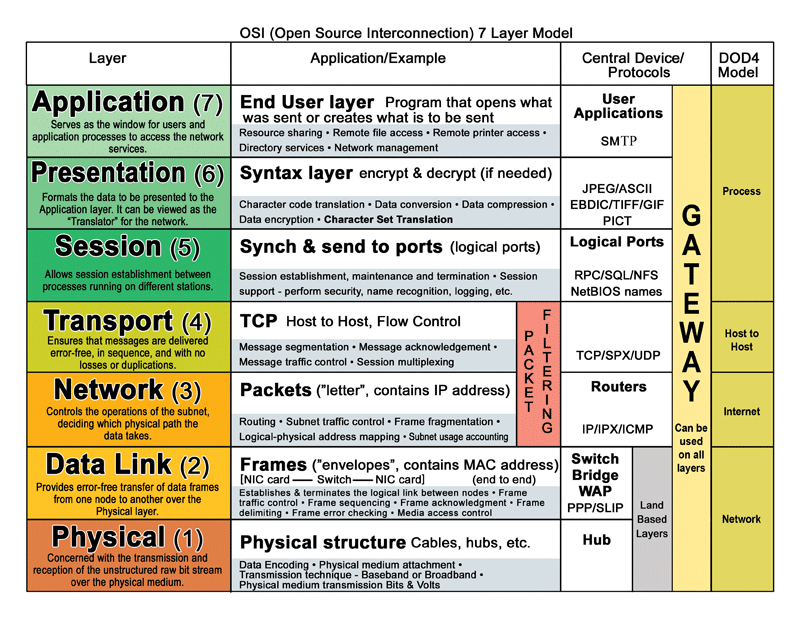
\includegraphics[width=0.9\linewidth,keepaspectratio]{../seminar1-intro/images/OSI-Model.png}
\end{center}

\end{frame}

\begin{frame}{OSI: уровни 1--3}
\begin{itemize}
  \item \textbf{L1 --- Physical (физический)}
  \begin{itemize}
    \item Передача битов по физической среде (кабель, радиоволны, оптика)
    \item Примеры: Ethernet PHY, Wi-Fi (802.11) физика, USB
    \item Понятий «адресации» нет --- только сигналы
  \end{itemize}
  \item \textbf{L2 --- Data Link (канальный)}
  \begin{itemize}
    \item Передача кадров (frames) между узлами в пределах одного сегмента сети
    \item Адресация: MAC-адреса (48 бит)
    \item Примеры: Ethernet (802.3), Wi-Fi (802.11), PPP, VLAN
    \item Контроль ошибок и коллизий (CSMA/CD, CSMA/CA)
  \end{itemize}
  \item \textbf{L3 --- Network (сетевой)}
  \begin{itemize}
    \item Маршрутизация пакетов между сетями
    \item Адресация: IP-адреса (IPv4/IPv6)
    \item Примеры: IP, ICMP (\texttt{ping}), протоколы маршрутизации (OSPF, BGP)
    \item Не гарантирует доставку, порядок, отсутствие дубликатов
  \end{itemize}
\end{itemize}
\end{frame}

\begin{frame}
\frametitle{Время вычислять по IP}

Вопрос: можно ли определить наше местоположение по IP-адресу?
% Да, через GeoIP базы, т.е. какие-то признаки, которые ассоциируются с географическими регионами (например, код страны, провайдера, города).

\begin{center}

\includegraphics[width=0.5\linewidth,keepaspectratio]{images/ip-meme.jpg}
\end{center}

\end{frame}

\begin{frame}{OSI L4 --- Transport (транспортный уровень)}
\textbf{Задача:} обеспечить логический канал между процессами (не машинами).
\begin{itemize}
  \item Адресация: \textbf{порты} (0--65535) идентифицируют процесс на хосте
  \item Два главных протокола: \textbf{TCP} и \textbf{UDP}
\end{itemize}
\vspace{0.3cm}
\begin{center}
\begin{tabular}{lll}
\textbf{Свойство}       & \textbf{TCP}                       & \textbf{UDP}              \\ \hline
Установка соединения    & Да (3-way handshake)               & Нет                       \\
Гарантия доставки       & Да (ACK + retransmit)              & Нет                       \\
Порядок пакетов         & Да                                 & Нет                       \\
Контроль потока         & Да (sliding window)                & Нет                       \\
Overhead заголовка      & 20+ байт                           & 8 байт                    \\
Задержка                & Выше                               & Ниже                      \\
\end{tabular}
\end{center}
\end{frame}

\begin{frame}{TCP --- как устроено надёжное соединение}
\begin{itemize}
  \item \textbf{3-way handshake}: SYN $\to$ SYN-ACK $\to$ ACK (установка соединения)
  \item \textbf{4-way teardown}: FIN $\to$ ACK $\to$ FIN $\to$ ACK (закрытие)
  \item \textbf{Sequence numbers}: каждый байт пронумерован; получатель отправляет ACK
  \item \textbf{Retransmission}: при отсутствии ACK --- повторная отправка (timeout / fast retransmit)
  \item \textbf{Sliding window}: отправитель посылает несколько сегментов без ожидания ACK
  \item \textbf{Congestion control}: алгоритмы (CUBIC, BBR) предотвращают перегрузку сети
\end{itemize}
\vspace{0.3cm}
\textbf{Следствие для распределённых систем:} TCP скрывает потери, но не скрывает \textbf{задержки} и не защищает от \textbf{head-of-line blocking} (пакет потерян --- вся очередь ждёт).
\end{frame}

\begin{frame}
\frametitle{Заголовок TCP-пакета}
\begin{center}
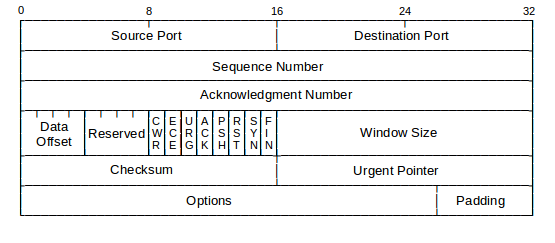
\includegraphics[width=0.9\linewidth,keepaspectratio]{images/tcp_header.png}
% source: https://intronetworks.cs.luc.edu/1/html/tcp.html
\end{center}
\begin{itemize}\tiny
  \item \textbf{Source/Destination Port} --- идентификаторы процессов на отправителе и получателе
  \item \textbf{Sequence Number} --- номер первого байта в сегменте (база для упорядочивания и повторной отправки)
  \item \textbf{Acknowledgment Number} --- подтверждение: \texttt{ACK = N} означает, что получены все байты до \texttt{N-1}
  \item \textbf{Flags} (SYN, ACK, FIN, RST, PSH, URG) --- управление жизненным циклом соединения
  \item \textbf{Window Size} --- сколько байт получатель готов принять (flow control)
  \item \textbf{Checksum} --- контроль целостности заголовка и данных
\end{itemize}
\end{frame}

\begin{frame}
\frametitle{Handshake \& Teardown}
\begin{center}
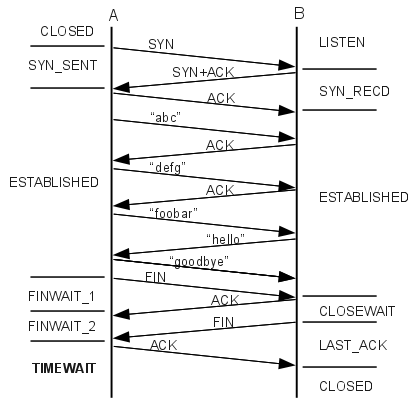
\includegraphics[width=0.65\linewidth,keepaspectratio]{images/tcp_ladder_states.png}
% source: https://intronetworks.cs.luc.edu/1/html/tcp.html
\end{center}
\end{frame}

\begin{frame}
\frametitle{Head-of-line blocking}
\begin{center}
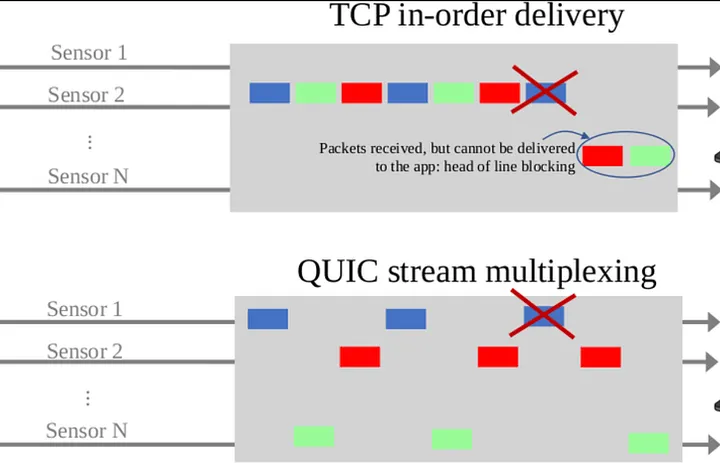
\includegraphics[width=0.65\linewidth,keepaspectratio]{images/hol-blocking.png}
% source: https://medium.com/@aditimishra_541/head-of-line-blocking-explanation-and-designing-a-flexible-network-layer-a1b44cde01be
\end{center}
\end{frame}

\begin{frame}{UDP --- когда отказываются от гарантий}
\begin{itemize}
  \item Нет соединения, нет ACK, нет порядка --- \emph{fire-and-forget}
  \item \textbf{Где это уместно:}
  \begin{itemize}
    \item DNS (один short запрос/ответ, retransmit на application level)
    \item Стриминг видео/аудио (устаревший пакет бесполезен)
    \item Онлайн-игры (позиция игрока --- нужна свежая, а не старая)
    \item QUIC (HTTP/3) --- реализует надёжность поверх UDP для устранения head-of-line blocking TCP
  \end{itemize}
  \item \textbf{Главное преимущество:} минимальная задержка и управление на уровне приложения
  \item Multicast и broadcast возможны только через UDP
\end{itemize}
\end{frame}

\begin{frame}
\frametitle{Заголовок UDP-пакета}

\begin{center}
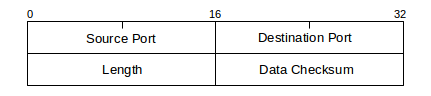
\includegraphics[width=0.9\linewidth,keepaspectratio]{images/udp_header.png}
% source: https://intronetworks.cs.luc.edu/1/html/udp.html
\end{center}

\begin{itemize}
  \item \textbf{Source/Destination Port} --- порты приложений отправителя и получателя
  \item \textbf{Length} --- длина UDP-датаграммы в байтах (заголовок + payload)
  \item \textbf{Checksum} --- контроль целостности заголовка и данных (в IPv6 обязателен)
  \item Заголовок очень маленький (8 байт): нет sequence number, ACK, окна, флагов
  \item Поэтому UDP быстрый и простой, но надёжность/порядок при необходимости реализуются на уровне приложения
\end{itemize}

\end{frame}

\section{Античность: CORBA и EJB}

\begin{frame}{Античность на примерах: где это реально жило}
\begin{itemize}
  \item \textbf{Банки:} карточный процессинг, платёжный шлюз, anti-fraud как отдельные удалённые сервисы
  \item \textbf{Телеком:} биллинг, CRM, provisioning, сеть IN через enterprise bus
  \item \textbf{Гос-системы:} тяжёлые интеграции между ведомствами через централизованные middleware
\end{itemize}
\begin{block}{Типичный стек конца 90-х / начала 2000-х}
App Server (WebLogic/WebSphere/JBoss) + ORB/CORBA + EJB + Oracle DB + JMS.
\end{block}
\end{frame}

\begin{frame}[fragile]{CORBA: пример IDL-контракта}
\begin{minted}[fontsize=\small]{idl}
module bank {
  interface PaymentService {
    string pay(in string accountId,
               in double amount,
               in string currency);
  };
};
\end{minted}
\begin{itemize}
  \item Из IDL генерировались стабы/скелетоны для C++/Java
  \item Клиент видел вызов как обычный метод, но под капотом шёл IIOP
  \item Контракт строгий: несовместимые изменения ломают клиентов
\end{itemize}
\end{frame}


\begin{frame}
\frametitle{Ох уж эта CORBA}

\begin{center}
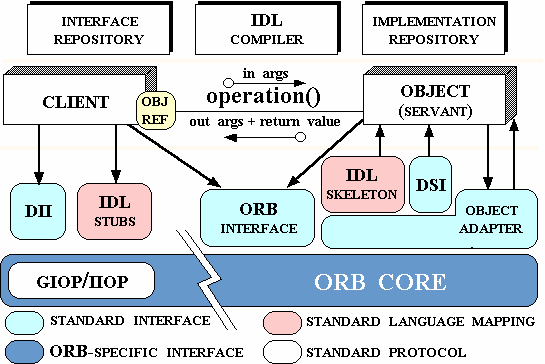
\includegraphics[width=1.0\linewidth,keepaspectratio]{images/corba5.png}
% https://www.dre.vanderbilt.edu/~schmidt/corba-overview.html
\end{center}

\end{frame}

\begin{frame}[fragile]{CORBA: как выглядел вызов}
\begin{minted}[fontsize=\small]{java}
org.omg.CORBA.Object ref =
    orb.string_to_object(ior);
PaymentService svc =
    PaymentServiceHelper.narrow(ref);

String txId = svc.pay("ACC-42", 199.99, "RUB");
\end{minted}
\begin{itemize}
  \item \texttt{narrow(...)} --- приведение к нужному удалённому интерфейсу
  \item IOR/Naming Service --- как клиент находит удалённый объект
  \item Ошибки часто проявлялись как таймауты ORB и проблемы совместимости версий
\end{itemize}
\end{frame}

\begin{frame}[fragile]{EJB: минимальный пример бизнес-бина}
\begin{minted}[fontsize=\small]{java}
@Stateless
public class PaymentBean {
  @PersistenceContext EntityManager em;

  @TransactionAttribute(REQUIRED)
  public String pay(String accountId, BigDecimal amount) {
    // списание, запись транзакции, аудит
    return UUID.randomUUID().toString();
  }
}
\end{minted}
\begin{itemize}
  \item Транзакция открывается контейнером автоматически
  \item Без ручного JDBC begin/commit/rollback в бизнес-коде
\end{itemize}
\end{frame}

\begin{frame}[fragile]{EJB: асинхронная обработка через MDB}
\begin{minted}[fontsize=\small]{java}
@MessageDriven(activationConfig = {
  @ActivationConfigProperty(
    propertyName = "destination",
    propertyValue = "jms/PaymentsQueue")
})
public class FraudCheckMDB implements MessageListener {
  public void onMessage(Message msg) {
    // anti-fraud проверка транзакции
  }
}
\end{minted}
\begin{itemize}
  \item Практический пайплайн: API $\to$ JMS Queue $\to$ MDB worker
  \item Ретраи, dead-letter и pooling часто настраивались на уровне контейнера
\end{itemize}
\end{frame}

\begin{frame}{Античные паттерны в современном виде}
\begin{center}
\begin{tabular}{ll}
\textbf{Тогда}                     & \textbf{Сейчас}                         \\ \hline
CORBA IDL + IIOP                   & gRPC + protobuf + HTTP/2                \\
EJB Stateless Bean                 & Spring Service / Micronaut Bean         \\
EJB TransactionAttribute           & @Transactional в современных фреймворках\\
Message-Driven Bean + JMS          & Kafka/RabbitMQ consumer                 \\
App Server clustering              & Kubernetes + service mesh               \\
\end{tabular}
\end{center}
\vspace{0.3cm}
\textbf{Вывод:} подходы не исчезли, они переродились в более лёгких и web-native инструментах.
\end{frame}


\section{Барокко: REST и SOAP}

\begin{frame}{REST --- Representational State Transfer}
\begin{itemize}
  \item REST --- архитектурный стиль для распределённых гипермедиа-систем, описан Roy Fielding в диссертации (2000)
  \item Не протокол, а набор \textbf{архитектурных ограничений} поверх HTTP
\end{itemize}
\begin{block}{Ключевые понятия}
\begin{itemize}
  \item \textbf{Ресурс} --- любая именованная сущность (пользователь, заказ, документ)
  \item \textbf{Представление} --- сериализованное состояние ресурса: JSON, XML, ...
  \item \textbf{URI} --- унифицированный идентификатор ресурса (\texttt{/users/42})
\end{itemize}
\end{block}
\end{frame}

\begin{frame}{Принципы REST}
\begin{enumerate}
  \item \textbf{Client--Server} --- разделение ответственности: клиент управляет UI, сервер --- данными
  \item \textbf{Stateless} --- каждый запрос содержит всю необходимую информацию; сессионное состояние хранится на клиенте
  \item \textbf{Cacheable} --- ответы явно указывают, можно ли их кэшировать
  \item \textbf{Uniform Interface} --- единый интерфейс: идентификация ресурсов через URI, манипуляция через представления, HATEOAS
  \item \textbf{Layered System} --- клиент не знает, общается ли он с конечным узлом или промежуточным (балансировщик, кэш)
  \item \textbf{Code on Demand} {\small (опционально)} --- сервер может передавать исполняемый код
\end{enumerate}
\end{frame}

\begin{frame}{HTTP методы}
\begin{center}
\begin{tabular}{llll}
\textbf{Метод} & \textbf{Idempotent} & \textbf{Safe} & \textbf{Использование} \\ \hline
\texttt{GET}    & Да  & Да  & Получить ресурс \\
\texttt{HEAD}   & Да  & Да  & Получить только заголовки \\
\texttt{POST}   & Нет & Нет & Создать ресурс / вызов действия \\
\texttt{PUT}    & Да  & Нет & Заменить ресурс целиком \\
\texttt{PATCH}  & Нет & Нет & Частично обновить ресурс \\
\texttt{DELETE} & Да  & Нет & Удалить ресурс \\
\end{tabular}
\end{center}
\vspace{0.3cm}
\textbf{Safe} --- не меняет состояние сервера \\
\textbf{Idempotent} --- повторный запрос даёт тот же результат
\end{frame}

\begin{frame}{HTTP статус-коды}
\begin{itemize}
  \item \textbf{2xx --- Success}: \texttt{200 OK}, \texttt{201 Created}, \texttt{204 No Content}
  \item \textbf{3xx --- Redirection}: \texttt{301 Moved Permanently}, \texttt{304 Not Modified}
  \item \textbf{4xx --- Client Error}:
  \begin{itemize}
    \item \texttt{400 Bad Request} --- неверный формат запроса
    \item \texttt{401 Unauthorized} --- требуется аутентификация
    \item \texttt{403 Forbidden} --- нет прав доступа
    \item \texttt{404 Not Found} --- ресурс не найден
    \item \texttt{409 Conflict} --- конфликт состояния (напр. дубликат)
    \item \texttt{429 Too Many Requests} --- rate limiting
  \end{itemize}
  \item \textbf{5xx --- Server Error}: \texttt{500 Internal Server Error}, \texttt{502 Bad Gateway}, \texttt{503 Service Unavailable}
\end{itemize}
\end{frame}

\begin{frame}[fragile]{REST --- форматы данных}
Чаще всего используется JSON, реже XML или другие форматы.
\begin{columns}
\column{0.5\textwidth}
\begin{minted}[fontsize=\small]{json}
{
  "id": 42,
  "name": "Alice",
  "email": "alice@example.com",
  "roles": ["admin", "user"]
}
\end{minted}
\column{0.5\textwidth}
\begin{minted}[fontsize=\small]{xml}
<user>
  <id>42</id>
  <name>Alice</name>
  <email>
    alice@example.com
  </email>
</user>
\end{minted}
\end{columns}
\vspace{0.3cm}
Content negotiation: клиент указывает предпочтительный формат через заголовки \texttt{Accept} и \texttt{Content-Type}.
\end{frame}

\begin{frame}{REST --- поддержание совместимости}
Как не сломать клиентов при изменении API?
\begin{itemize}
  \item \textbf{URL-версионирование} --- \texttt{/api/v1/users}, \texttt{/api/v2/users}
  \begin{itemize}
    \item Просто и явно, но засоряет URL-пространство
  \end{itemize}
  \item \textbf{Header-версионирование} --- \texttt{Accept: application/vnd.api+json;version=2}
  \begin{itemize}
    \item Чище по духу REST, но сложнее для клиентов и кэшей
  \end{itemize}
  \item \textbf{Эволюция схемы без сломки (non-breaking changes):}
  \begin{itemize}
    \item Добавлять новые поля можно --- клиенты игнорируют неизвестные поля
    \item Новые поля должны быть опциональными
    \item Не удалять и не переименовывать существующие поля
    \item Помечать deprecated-поля и поддерживать несколько версий до удаления
  \end{itemize}
\end{itemize}
\end{frame}

\begin{frame}{SOA и SOAP}
\begin{block}{SOA --- Service-Oriented Architecture}
  Архитектурный подход, при котором функциональность системы разбивается на сервисы, взаимодействующие через формально определённые интерфейсы.
\end{block}
\vspace{0.3cm}
\textbf{SOAP} (Simple Object Access Protocol) --- протокол обмена сообщениями на основе XML, типичный транспорт SOA-систем.
\begin{itemize}
  \item Разработан Microsoft, IBM и др. (1998), стандарт W3C
  \item Поддерживает разные транспорты: HTTP, SMTP, JMS, TCP
  \item Строгая типизация и контракт через \textbf{WSDL}
  \item Встроенные WS-стандарты: безопасность (WS-Security), транзакции (WS-AtomicTransaction), надёжная доставка (WS-ReliableMessaging)
\end{itemize}
\end{frame}

\begin{frame}[fragile]{SOAP --- структура сообщения}
\begin{minted}[fontsize=\scriptsize]{xml}
<soap:Envelope
    xmlns:soap="http://www.w3.org/2003/05/soap-envelope"
    xmlns:m="http://example.org/stock">
  <soap:Header>
    <m:Auth>
      <m:token>secret-token-123</m:token>
    </m:Auth>
  </soap:Header>
  <soap:Body>
    <m:GetStockPrice>
      <m:StockName>AAPL</m:StockName>
    </m:GetStockPrice>
  </soap:Body>
</soap:Envelope>
\end{minted}
\begin{itemize}
  \item \textbf{Envelope} --- обёртка, определяет содержимое как SOAP-сообщение
  \item \textbf{Header} --- метаданные: аутентификация, транзакции, маршрутизация
  \item \textbf{Body} --- основная полезная нагрузка (payload); \textbf{Fault} --- описание ошибки
\end{itemize}
\end{frame}

\begin{frame}[fragile]{WSDL --- Web Services Description Language}
WSDL --- XML-язык описания интерфейса веб-сервиса (аналог header-файла в C).
\begin{minted}[fontsize=\scriptsize]{xml}
<definitions name="StockQuote"
    targetNamespace="http://example.org/stock">
  <message name="GetPriceInput">
    <part name="symbol" type="xsd:string"/>
  </message>
  <message name="GetPriceOutput">
    <part name="price"  type="xsd:float"/>
  </message>
  <portType name="StockQuotePortType">
    <operation name="GetPrice">
      <input  message="GetPriceInput"/>
      <output message="GetPriceOutput"/>
    </operation>
  </portType>
</definitions>
\end{minted}
\textbf{Совместимость:} изменение WSDL требует новой версии контракта; клиенты перегенерируют стабы (\texttt{wsdl2java}, \texttt{wsimport}).
\end{frame}

\begin{frame}{REST vs SOAP}
\begin{center}
\begin{tabular}{lll}
\textbf{Критерий}      & \textbf{REST}          & \textbf{SOAP}                \\ \hline
Транспорт              & HTTP                   & HTTP, SMTP, TCP, ...         \\
Формат данных          & JSON, XML, ...         & XML (только)                 \\
Контракт               & OpenAPI / Swagger      & WSDL (строгий)               \\
Безопасность           & HTTPS, OAuth\,2.0      & WS-Security                  \\
Производительность     & Выше                   & Ниже                         \\
Типизация              & Слабая                 & Строгая                      \\
Применение             & Публичные API, web     & Корпоративный сектор         \\
\end{tabular}
\end{center}
\vspace{0.3cm}
REST --- для большинства новых проектов. SOAP --- когда нужны встроенные стандарты надёжности, безопасности и транзакционности.
\end{frame}

\section{Классицизм: gRPC, Thrift, Java RMI, ...}

\begin{frame}{Remote Procedure Call (RPC)}
\begin{block}{Идея}
  Вызов удалённой функции должен выглядеть как вызов локальной функции.
\end{block}
\begin{itemize}
  \item \textbf{Stub / Proxy} --- локальный объект, перехватывающий вызов
  \item \textbf{Marshalling} --- преобразование аргументов в байты для передачи
  \item \textbf{Transport} --- доставка сообщения по сети
  \item \textbf{Unmarshalling} --- восстановление аргументов на стороне сервера
\end{itemize}
\vspace{0.3cm}
\textbf{Фундаментальная проблема RPC --- частичные отказы:}
\begin{itemize}
  \item Запрос дошёл, ответ --- нет: выполнилось ли?
  \item Ответ пришёл с задержкой: нужна идемпотентность
  \item Сервер недоступен: нужны retry, circuit breaker, timeout
\end{itemize}
\end{frame}

\begin{frame}[fragile]{gRPC --- определение и .proto}
\begin{itemize}
  \item \textbf{gRPC} --- RPC-фреймворк от Google (2015); использует \textbf{Protocol Buffers} для сериализации и \textbf{HTTP/2} в качестве транспорта
  \item Поддерживает: C++, Java, Go, Python, Rust, Node.js, C\#, Ruby, ...
\end{itemize}
\begin{minted}[fontsize=\small]{protobuf}
syntax = "proto3";
service UserService {
  rpc GetUser   (GetUserRequest)   returns (User);
  rpc ListUsers (ListUsersRequest) returns (stream User);
}
message GetUserRequest { int64 id = 1; }
message User {
  int64  id    = 1;
  string name  = 2;
  string email = 3;
}
\end{minted}
\end{frame}

\begin{frame}{gRPC --- forward/backward совместимость}
Protocol Buffers обеспечивает совместимость через \textbf{номера полей} (field numbers).
\begin{itemize}
  \item \textbf{Backward compatibility} --- новый сервер понимает старых клиентов:
  \begin{itemize}
    \item Можно добавлять новые поля; старые клиенты их не заполняют --- сервер видит значения по умолчанию
  \end{itemize}
  \item \textbf{Forward compatibility} --- старый сервер понимает новых клиентов:
  \begin{itemize}
    \item Неизвестные поля игнорируются (proto3)
  \end{itemize}
  \item \textbf{Запрещено:} удалять или переиспользовать \textbf{номера полей}; менять тип поля
  \item \textbf{Рекомендуется:} при удалении поля помечать его номер как \texttt{reserved}
\end{itemize}
\vspace{0.2cm}
\textbf{Итог:} клиент и сервер можно обновлять независимо (independent deployability).
\end{frame}

\begin{frame}{gRPC --- производительность и HTTP/2}
\begin{itemize}
  \item \textbf{Бинарная сериализация} (protobuf) --- в 3--10$\times$ компактнее JSON
  \item \textbf{HTTP/2 мультиплексирование} --- множество запросов в одном TCP-соединении без head-of-line blocking
  \item \textbf{Header compression} (HPACK) --- экономия трафика
  \item \textbf{Стриминг} --- 4 режима взаимодействия:
  \begin{itemize}
    \item Unary (1 запрос $\to$ 1 ответ, аналог обычного HTTP)
    \item Server streaming (1 запрос $\to$ поток ответов)
    \item Client streaming (поток запросов $\to$ 1 ответ)
    \item Bidirectional streaming (поток $\leftrightarrow$ поток)
  \end{itemize}
  \item Встроены: deadlines/timeouts, cancellation, metadata, interceptors
\end{itemize}
\end{frame}

\begin{frame}[fragile]{Apache Thrift}
\begin{itemize}
  \item Разработан в Facebook (2007), передан в Apache Foundation
  \item Генерирует код из \textbf{IDL} (.thrift) для 25+ языков: Java, C++, Python, Go, Ruby, Erlang, Haskell, ...
\end{itemize}
\begin{minted}[fontsize=\small]{thrift}
namespace java org.example

struct User {
  1: i64    id,
  2: string name,
  3: optional string email
}

service UserService {
  User       getUser  (1: i64 id),
  list<User> listUsers()
}
\end{minted}
\end{frame}

\begin{frame}{Thrift --- протоколы и транспорты}
Thrift разделяет \textbf{протокол} (сериализацию) и \textbf{транспорт} независимо:
\begin{columns}
\column{0.5\textwidth}
\textbf{Протоколы:}
\begin{itemize}
  \item \texttt{BinaryProtocol} --- компактный бинарный
  \item \texttt{CompactProtocol} --- variable-length encoding, ещё меньше
  \item \texttt{JSONProtocol} --- JSON для отладки и веб-интеграции
\end{itemize}

\column{0.5\textwidth}
\textbf{Транспорты:}
\begin{itemize}
  \item \texttt{TSocket} --- TCP
  \item \texttt{THttpClient} --- HTTP
  \item \texttt{TMemoryBuffer} --- in-memory (тесты)
  \item \texttt{TFramedTransport} --- обёртка для async
\end{itemize}
\end{columns}
\vspace{0.3cm}
\textbf{Совместимость:} аналогично protobuf --- номера полей обеспечивают совместимость; \texttt{optional} поля можно добавлять без сломки клиентов.
\end{frame}

\begin{frame}{gRPC vs Thrift}
\begin{center}
\begin{tabular}{lll}
\textbf{Критерий}       & \textbf{gRPC}         & \textbf{Thrift}            \\ \hline
Основатель              & Google                & Facebook (Apache)          \\
Транспорт               & HTTP/2 (только)       & TCP, HTTP, memory, ...     \\
Сериализация            & protobuf (только)     & binary, compact, JSON      \\
Поддержка языков        & $\approx$12           & $\approx$28                \\
Стриминг                & Встроенный (4 вида)   & Нет                        \\
Популярность сейчас     & Выше                  & Ниже                       \\
\end{tabular}
\end{center}
\vspace{0.3cm}
\textbf{Когда Thrift?} Если нужна поддержка экзотических языков или гибкость транспорта, либо работаете в экосистеме, где Thrift уже используется (HBase, Scribe и др.).
\end{frame}

\begin{frame}{Java RMI}
\textbf{Java Remote Method Invocation} --- встроенный механизм RPC для Java (JDK 1.1, 1997).
\begin{itemize}
  \item Позволяет вызывать методы объектов на другой JVM как локальные
  \item Архитектура:
  \begin{itemize}
    \item \textbf{Remote Interface} --- интерфейс, расширяющий \texttt{java.rmi.Remote}
    \item \textbf{Stub} --- заглушка на стороне клиента (генерируется автоматически)
    \item \textbf{RMI Registry} --- сервис имён для поиска объектов (\texttt{rmiregistry})
  \end{itemize}
  \item Передаёт аргументы через \textbf{Java Serialization}
  \item Ограничения:
  \begin{itemize}
    \item Только Java
    \item Медленная и небезопасная десериализация (CVE)
    \item Проблемы с firewall (динамические порты)
    \item Практически вытеснен gRPC/Thrift в современных системах
  \end{itemize}
\end{itemize}
\end{frame}

\begin{frame}[fragile]{Java RMI --- пример}
\begin{minted}[fontsize=\small]{java}
// 1. Remote Interface
public interface Hello extends Remote {
    String sayHello() throws RemoteException;
}

// 2. Server: publish the object
HelloImpl obj = new HelloImpl();
Hello stub = (Hello) UnicastRemoteObject
        .exportObject(obj, 0);
Registry registry = LocateRegistry.getRegistry();
registry.bind("Hello", stub);

// 3. Client: lookup and invoke
Registry registry =
        LocateRegistry.getRegistry("host");
Hello stub = (Hello) registry.lookup("Hello");
String response = stub.sayHello(); // remote call!
\end{minted}
\end{frame}

\section{Модернизм: очереди сообщений}

\begin{frame}{Что такое очередь сообщений?}
\begin{block}{Message Queue}
  Посредник между продюсерами и консюмерами, который принимает сообщения, временно хранит их и доставляет получателям.
\end{block}
\begin{itemize}
  \item \textbf{Decoupling по времени}: отправитель и получатель не обязаны быть онлайн одновременно
  \item \textbf{Decoupling по нагрузке}: очередь сглаживает пики входящего трафика
  \item \textbf{Async processing}: медленные задачи выносятся в фон
  \item \textbf{Fan-out}: одно сообщение может быть доставлено нескольким подписчикам
\end{itemize}
\vspace{0.3cm}
\textbf{Типичный pipeline:} API принимает запрос $\to$ кладёт задачу в очередь $\to$ worker обрабатывает $\to$ пишет результат в БД.
\end{frame}

\begin{frame}{Семантики доставки}
\begin{itemize}
  \item \textbf{At-most-once}
  \begin{itemize}
    \item Сообщение доставляется не более одного раза
    \item Потери возможны, дубликатов почти нет
  \end{itemize}
  \item \textbf{At-least-once}
  \begin{itemize}
    \item Сообщение будет доставлено, но может прийти повторно
    \item Требуется \textbf{idempotent} обработчик
  \end{itemize}
  \item \textbf{Exactly-once} (в узком контексте)
  \begin{itemize}
    \item Сложно и дорого в распределённых системах
    \item Обычно реализуется как комбинация идемпотентности, транзакций и deduplication
  \end{itemize}
\end{itemize}
\end{frame}

\begin{frame}{Kafka --- что это?}
\textbf{Apache Kafka} --- distributed commit log для потоковой передачи событий.
\begin{itemize}
  \item Изначально создан в LinkedIn (2011), сейчас проект Apache
  \item Основная абстракция --- \textbf{topic}, разбитый на \textbf{partitions}
  \item Сообщения в партиции упорядочены по offset
  \item Продюсеры пишут в topic, консюмеры читают независимо
  \item Данные реплицируются между брокерами для отказоустойчивости
\end{itemize}
\begin{block}{Ментальная модель}
Kafka --- это не классическая FIFO-очередь, а \textbf{журнал событий}, где сообщения читаются как лог.
\end{block}
\end{frame}

\begin{frame}{Kafka --- архитектура и масштабирование}
\begin{itemize}
  \item \textbf{Broker} --- сервер Kafka, хранящий партиции
  \item \textbf{Topic} --- логическая категория событий
  \item \textbf{Partition} --- физический shard внутри topic
  \item \textbf{Replication factor} --- количество копий каждой партиции
  \item \textbf{Leader/Follower} --- запись и чтение обычно идут через лидера партиции
  \item \textbf{Consumer group} --- масштабирование чтения: каждая партиция читается только одним консюмером в группе
\end{itemize}
\vspace{0.2cm}
\textbf{Эффект:} throughput растёт при увеличении числа партиций и брокеров.
\end{frame}

\begin{frame}
\frametitle{Схема Kafka}

\begin{center}
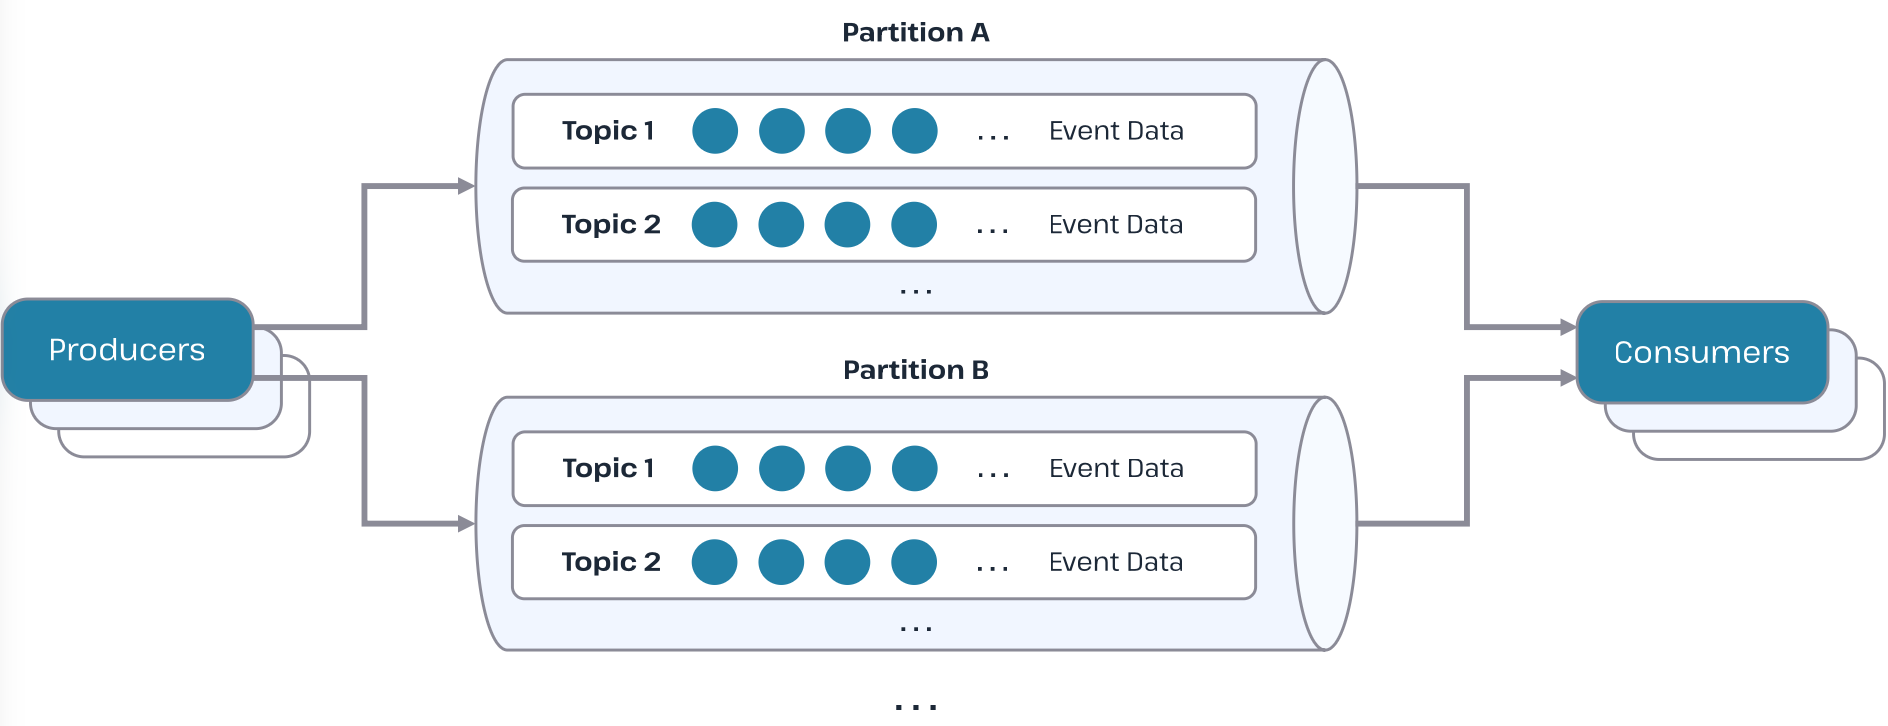
\includegraphics[width=1.0\linewidth,keepaspectratio]{images/diagram-apache-kafka.png}
% https://hazelcast.com/foundations/data-and-middleware-technologies/kafka/
\end{center}

\end{frame}

\begin{frame}{Kafka --- гарантии и порядок}
\begin{itemize}
  \item Порядок сообщений гарантируется \textbf{внутри одной partition}
  \item Между разными partition общий порядок не гарантируется
  \item Обычно используется \textbf{at-least-once} доставка
  \item Для строгой обработки полезны:
  \begin{itemize}
    \item idempotent producer (без дубликатов при retry)
    \item transactional producer/consumer (EOS в рамках Kafka pipeline)
    \item ручное управление commit offset
  \end{itemize}
  \item Retention-based хранение: сообщения живут по времени или объёму, а не до подтверждения потребителем
\end{itemize}
\end{frame}

\begin{frame}{Kafka --- где особенно хороша}
\begin{itemize}
  \item Event sourcing и event-driven архитектуры
  \item Сбор логов и телеметрии (ELK, observability)
  \item Потоковая обработка (Kafka Streams, Flink, Spark)
  \item Интеграция микросервисов через immutable events
\end{itemize}
\vspace{0.3cm}
\textbf{Плюсы:}
\begin{itemize}
  \item Очень высокий throughput и горизонтальное масштабирование
  \item Долговременное хранение и повторное чтение истории
\end{itemize}
\textbf{Минусы:}
\begin{itemize}
  \item Более высокий порог входа в эксплуатацию
  \item Не лучшая модель для сложной маршрутизации единичных задач
\end{itemize}
\end{frame}

\begin{frame}{RabbitMQ --- что это?}
\textbf{RabbitMQ} --- брокер сообщений на базе протокола AMQP (классическая message queue).
\begin{itemize}
  \item Ядро написано на Erlang (высокая надёжность и конкурентность)
  \item Основные сущности: \textbf{exchange}, \textbf{queue}, \textbf{binding}
  \item Продюсер публикует сообщение в exchange
  \item Exchange маршрутизирует сообщение в очереди по правилам binding
  \item Консюмеры получают сообщения из очередей и отправляют \texttt{ack}
\end{itemize}
\end{frame}

\begin{frame}{RabbitMQ --- маршрутизация и паттерны}
\begin{itemize}
  \item \textbf{Типы exchange:}
  \begin{itemize}
    \item \texttt{direct} --- по точному routing key
    \item \texttt{topic} --- по шаблону (\texttt{order.*}, \texttt{*.created})
    \item \texttt{fanout} --- широковещательная рассылка всем связанным очередям
    \item \texttt{headers} --- по заголовкам сообщения
  \end{itemize}
  \item \textbf{Популярные паттерны:}
  \begin{itemize}
    \item Work queue (распределение задач по воркерам)
    \item Pub/Sub (fanout exchange)
    \item RPC over MQ (request-reply)
    \item Dead-letter queue (DLQ) для неуспешных сообщений
  \end{itemize}
\end{itemize}
\end{frame}

\begin{frame}
\frametitle{Схема RabbitMQ}

\begin{center}
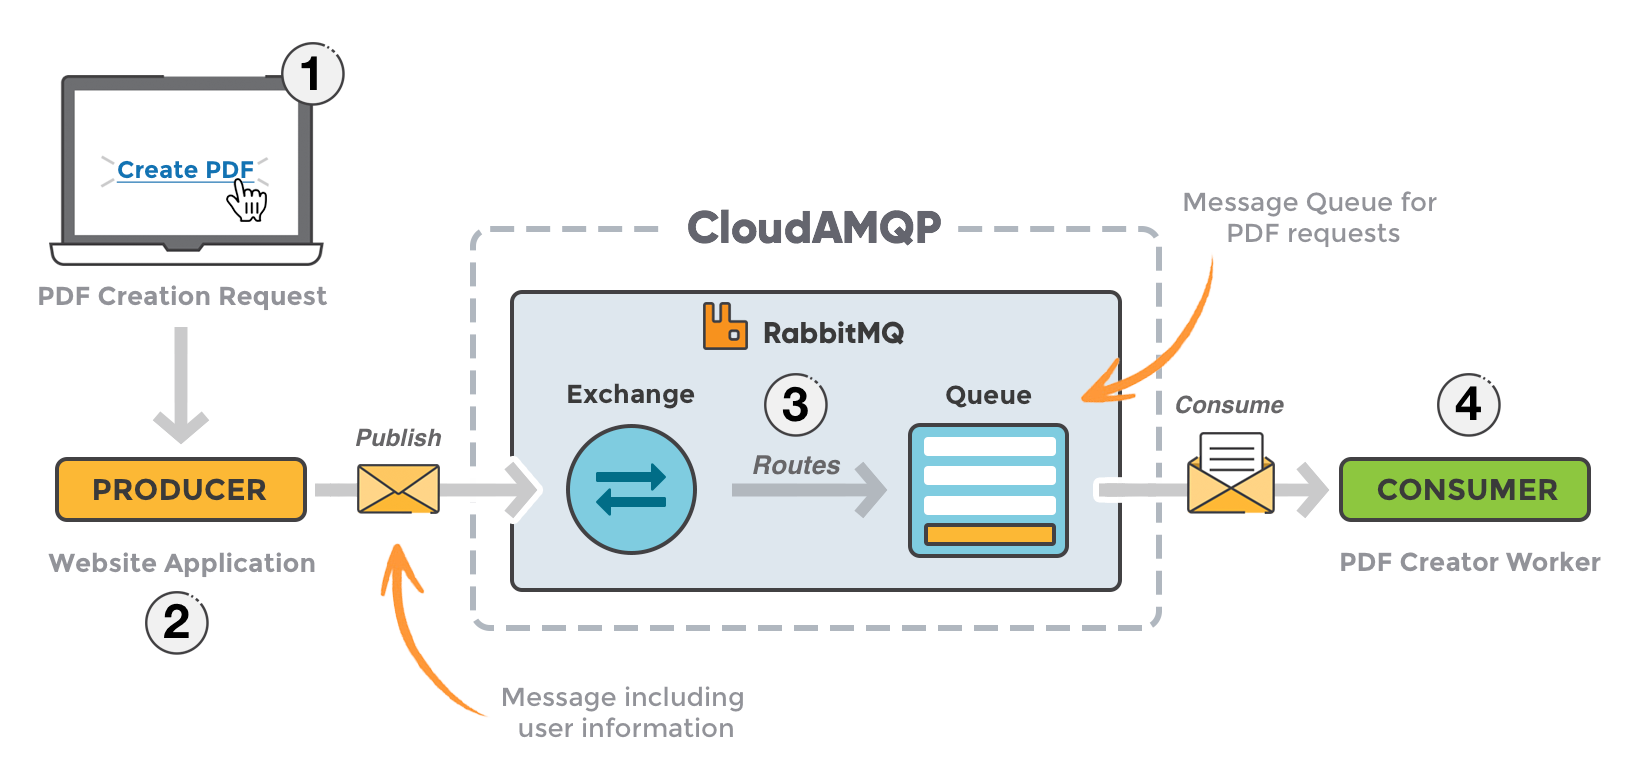
\includegraphics[width=1.0\linewidth,keepaspectratio]{images/rabbitmq-beginners-updated.png}
% https://hazelcast.com/foundations/data-and-middleware-technologies/rabbitmq/
\end{center}

\end{frame}

\begin{frame}{RabbitMQ --- надёжность и эксплуатация}
\begin{itemize}
  \item \textbf{Ack/Nack} --- явное подтверждение обработки сообщения
  \item \textbf{Durable queue + persistent messages} --- переживают перезапуск брокера
  \item \textbf{Prefetch (QoS)} --- ограничивает число сообщений на консюмера
  \item \textbf{TTL} и \textbf{DLX} --- политика повторов и отбраковки
  \item \textbf{Quorum queues} --- современная отказоустойчивая реализация очередей
\end{itemize}
\vspace{0.3cm}
\textbf{Сильная сторона RabbitMQ:} гибкая маршрутизация и удобство для task queue сценариев.
\end{frame}

\begin{frame}{Kafka vs RabbitMQ}
\begin{center}
\begin{tabular}{lll}
\textbf{Критерий}       & \textbf{Kafka}                        & \textbf{RabbitMQ}                  \\ \hline
Модель                 & Distributed log                        & Message broker / queues            \\
Хранение               & Retention (дни/недели)                & Обычно до доставки                 \\
Порядок                & Внутри partition                       & $\pm$ Внутри очереди       \\
Маршрутизация          & Topic/partition key                    & Exchange + bindings      \\
Throughput             & Очень высокий                         & $\pm$ Ниже      \\
Основной use-case      & Event streaming                       & Task queues, интеграции, RPC       \\
\end{tabular}
\end{center}
\vspace{0.2cm}
\textbf{Практика:} часто используют вместе: RabbitMQ --- для команд, интеграций и задач, Kafka --- для событий и аналитики.
\end{frame}

\section{Немного про тестирование распределенных систем}

\begin{frame}{Зачем тестировать распределённые системы?}
\begin{itemize}
  \item Распределённые системы отказывают не так, как монолиты: \textbf{частичные отказы}, \textbf{гонки}, \textbf{сетевые разбиения}
  \item Классические unit-тесты не воспроизводят сетевые аномалии
  \item Баги могут проявляться только под нагрузкой или при конкретном порядке событий
\end{itemize}
\begin{alertblock}{Знаменитые аварии}
\begin{itemize}
  \item \textbf{Amazon DynamoDB (2012)} --- потеря данных из-за ошибки в логике репликации
  \item \textbf{Cloudflare (2019)} --- каскадный отказ из-за ошибки в firewall-правилах
  \item \textbf{CockroachDB (2020)} --- нарушение serializability при concurrent транзакциях (найдено Jepsen)
\end{itemize}
\end{alertblock}
\end{frame}

\begin{frame}{Jepsen}
\begin{itemize}
  \item Создан Kyle Kingsbury (aphyr) в 2013 году, написан на Clojure
  \item Тестирует \textbf{согласованность} (consistency) и \textbf{доступность} распределённых баз данных
  \item \textbf{Принцип работы:}
  \begin{enumerate}
    \item Запускает кластер в Docker-контейнерах
    \item Параллельно выполняет операции чтения/записи через клиентов
    \item Одновременно вносит \textbf{немезиды} (\href{https://github.com/jepsen-io/jepsen/blob/main/doc/tutorial/05-nemesis.md}{nemeses}): network partitions, clock skew, kill nodes
    \item Собирает полную историю операций
    \item Проверяет историю на соответствие модели через алгоритмы \textbf{Elle} (serializability) и \textbf{Knossos} (linearizability)
  \end{enumerate}
  \item Нашёл критические баги в: Redis, Cassandra, ZooKeeper, MongoDB, CockroachDB, TiDB, HashiCorp Vault, ...
\end{itemize}
\end{frame}

\begin{frame}{Chaos Engineering}
\begin{block}{Chaos Engineering}
  Дисциплина проверки стойкости системы путём намеренного внесения отказов в production.
\end{block}
\begin{itemize}
  \item Принципы (Netflix):
  \begin{enumerate}
    \item Определить гипотезу о поведении системы в \emph{steady state}
    \item Намеренно вносить отказы: убивать узлы, вводить задержки, ошибки
    \item Наблюдать \textbf{отклонения} от steady state
    \item Повторять с возрастающим \emph{blast radius}
  \end{enumerate}
  \item Инструменты:
  \begin{itemize}
    \item \textbf{Chaos Monkey / Gorilla / Kong} (Netflix) --- убивают инстансы / AZ / регион
    \item \textbf{Gremlin} --- коммерческая платформа для chaos experiments
    \item \textbf{Chaos Mesh} --- для Kubernetes: network delay, pod kill, IO fault
    \item \textbf{toxiproxy} (Shopify) --- proxy для эмуляции сетевых проблем
  \end{itemize}
\end{itemize}
\end{frame}

\begin{frame}{Нагрузочное и стресс-тестирование}
\begin{itemize}
  \item \textbf{Load testing} --- поведение под \textbf{ожидаемой} нагрузкой
  \begin{itemize}
    \item Метрики: latency (p50/p95/p99), throughput (RPS), error rate
  \end{itemize}
  \item \textbf{Stress testing} --- ищем поведение при \textbf{превышении} нормальной нагрузки
  \begin{itemize}
    \item Деградирует ли система \emph{gracefully}?
  \end{itemize}
  \item \textbf{Soak testing} --- длительная нагрузка (утечки памяти, деградация соединений)
  \item \textbf{Spike testing} --- резкий всплеск нагрузки
\end{itemize}
\vspace{0.2cm}
\textbf{Инструменты:}
\begin{itemize}
  \item \textbf{k6} (Grafana) --- JavaScript DSL, удобен для CI/CD
  \item \textbf{Locust} --- Python DSL
  \item \textbf{Apache JMeter} --- GUI, широко используется в enterprise
  \item \textbf{wrk / wrk2} --- минималистичный HTTP-бенчмаркинг
\end{itemize}
\end{frame}

\begin{frame}{Фаззинг и формальные методы}
\begin{itemize}
  \item \textbf{Fuzzing} --- генерация случайных/мутированных входов для обнаружения падений и уязвимостей
  \begin{itemize}
    \item Применяется к: парсерам протоколов, сериализаторам, сетевым стекам
    \item Инструменты: AFL++, libFuzzer, go-fuzz, jazzer (JVM)
  \end{itemize}
  \item \textbf{Property-based testing} --- проверяем инварианты на случайно сгенерированных данных
  \begin{itemize}
    \item Инструменты: QuickCheck (Haskell), Hypothesis (Python), jqwik (Java)
  \end{itemize}
  \item \textbf{Model checking (формальная верификация):}
  \begin{itemize}
    \item \textbf{TLA+} (Lamport) --- используется в AWS S3, Azure Cosmos DB, FoundationDB
    \item \textbf{P language} (Microsoft) --- проверка распределённых протоколов
  \end{itemize}
\end{itemize}
\end{frame}


\begin{frame}
\frametitle{Итоги}

\begin{itemize}
  \item Вспомнили про стек OSI и сетевые аспекты взаимодействия
  \item Поговорили про способы организации взаимодействия между компонентами: REST, SOAP, gRPC, Thrift, RabbitMQ, Kafka
  \item gRPC, Docker (?), Thrift (?) будет посвящена вторая домашка (?)
\end{itemize}

\end{frame}

\end{document}